\documentclass{minimal}

\usepackage{graphicx}
\usepackage{tikz}
\usetikzlibrary{positioning}
\usetikzlibrary{shapes.geometric}

\begin{document}

\begin{tikzpicture}[
networknode/.style={regular polygon,regular polygon sides=4, draw=black, fill=none, very thick, inner sep=-7pt},
vectornode/.style={rectangle, draw=black, fill=none, very thick,},
imagenode/.style={rectangle, draw=none, fill=none},
]

\tikzstyle{line} = [draw, -latex']

%Nodes
% What sorta style should the text have? Blue ass well?
% mention a cnn somewhere
% also see https://www.researchgate.net/figure/The-high-level-concept-of-an-extended-variational-autoencoder-adopted-for_fig8_317486066
% http://bjlkeng.github.io/images/variational_autoencoder2.png
\node[imagenode] (input) [] [label=below:{$X$}]{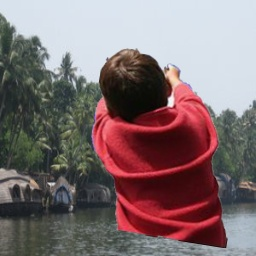
\includegraphics[width=0.2\textwidth]{syn1}};
\node[networknode] (encoder) [right=of input][label=below:{\mbox{$Q(z|X)$}}]{\textbf{Encoder Network}};
\node[vectornode] (latent) [right=of encoder] {$\sum^2{x+1}$};
\node[networknode] (decoder) [right=of latent][label=below:{\mbox{$P(X|z)$}}] {\textbf{Decoder Network}};
\node[imagenode] (output) [right=of decoder][label=below:$\widetilde{X}$] {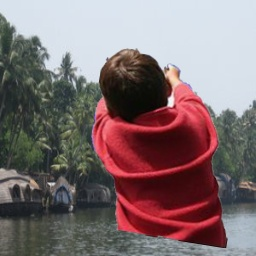
\includegraphics[width=0.2\textwidth]{syn1}};

%Lines
\draw[->] (input.east) -- (encoder.west);
%% \draw (encoder.south) node[label=below:$b_1$,draw]{}
\draw[->] (encoder.east) -- node [text width=2.5cm,midway,above] {convolutions} (latent.west) ;
\draw[->] (latent.east) -- (decoder.west);
\draw[->] (decoder.east) -- node [text width=2.5cm,midway,above] {transposed convolutions} (output.west);
%% \draw[->] (decoder.west) .. controls +(down:7mm) and +(right:7mm) .. (lowercircle.east);
%% \draw[->] (decoder.west) 

\end{tikzpicture}

\end{document}
